% copyright (c) 2018 Groupoid Infinity

\documentclass{article}
\usepackage{graphicx}
\usepackage{amsmath}
\usepackage{amssymb}
\usepackage{amsthm}
\usepackage{url}
\usepackage{tikz}
\usepackage{tikz-cd}
\usetikzlibrary{matrix}
\usetikzlibrary{babel}
\usepackage{listings}
\usepackage[numbers]{natbib}
\usepackage[utf8]{inputenc}
\theoremstyle{definition}
\newtheorem{definition}{Definition}
\newtheorem{theorem}{Theorem}

\def\mapright#1{\xrightarrow{{#1}}}
\def\mapleft#1{\xleftarrow{{#1}}}
\def\mapup#1{\Big\uparrow\rlap{\raise2pt{\scriptstyle{#1}}}}
\def\mapupl#1{\Big\uparrow\llap{\raise2pt{\scriptstyle{#1}}}}
\def\mapdown#1{\Big\downarrow\rlap{\raise2pt{\scriptstyle{#1}}}}
\def\mapdownl#1{\Big\downarrow\llap{\raise2pt{\scriptstyle{#1}}}}
\def\mapdiagl#1{\vcenter{\searrow}\rlap{\raise2pt{\scriptstyle{#1}}}}
\def\mapdiagr#1{\vcenter{\swarrow}\rlap{\raise2pt{\scriptstyle{#1}}}}

\lstset{basicstyle=\small,inputencoding=utf8}

\begin{document}

\title{Mathematical Components}
\author{Maxim Sokhatsky}
\date{
    $^1$ National Technical University of Ukraine \\
    \small Igor Sikorsky Kyiv Polytechnical Institute\\
    \today
}

\maketitle

\begin{abstract}

This seminar supposed to be a contemporary introduction
to modern type theory that is suitable for mathematicians needs,
in the sense that this theory forms a foundation of mathematics
and the language for theorems formulation and their proofs.

This course is dedicated to type checkers with cubical syntax, based on interval
with functional extensionality, higher equalities, and higher inductive types on
top of MLTT as a core. Please refer to CCHM paper for more information.
The base library used in this course is founded on top of cubical modules
each falling into one of 15 categories:

(i) MLTT Types: pi, sigma, path;
(ii) Set Theory: prop, set, ordinal, hedberg;
(iii) Run-Time Inductive Types: proto, maybe, bool, nat, list, stream, vector;
(iv) Abstract Algebra: algebra;
(v) Control Structures: control;
(vi) Recursion Schemes: recursion;
(vii) Univalent Foundations: equiv, retract, iso, univ;
(viii) Higher Inductive Types: interval, interval, s1, s2, pullback, pushout, suspension, quotient, trunc;
(ix) Process Calculus: process;
(x) Category Theory and Topos Theory: cat, fun, sip, adj, ump, cones, topos, category;
(xi) Contextual Categories: cwf, csystem;
(xii) Languages: mltt, infinity;
(xiii) Algebraic Geometry: pointed, euler, seq, hopf, cw;
(xiv) Cartan Geometry in Cohesive Topos: infinitesimal, etale, manifold, bundle, shape, sharp;
(xv) K-Theory: k\_theory, swaptrans, bishop, subtype;
This library is best to read with HoTT book and Felix Wellen dissertation.

{\bf Keywords}: Cubical Type Theory, Homotopy Type Theory, Category Theory, Topos Theory
\end{abstract}

\newpage
\tableofcontents
\newpage

\section*{Intro}
\subsection*{Cubical Syntax}

The BNF notation consists of 1) telescopes (contexts or sigma chains);
2) inductive data definitions (sum chains); 3) split eliminator;
4) branches of split eliminators; 5) pure dependent type theory syntax.
It also has where, import, module constructions.

\begin{lstlisting}[mathescape=true]
def := ${\bf data}$ id tele = sum + id tele : exp = exp +
       id tele : exp ${\bf where}$ def

exp := cotele*exp + cotele$\rightarrow$exp + exp$\rightarrow$exp + (exp) + app + id +
       (exp,exp) + \ cotele$\rightarrow$exp + ${\bf split}$ cobrs + exp${\bf.1}$ + exp${\bf.2}$
\end{lstlisting}

\begin{lstlisting}[mathescape=true]
     0 := #empty         imp    := [ ${\bf import}$ id ]
   brs := 0 + cobrs      tele   := 0 + cotele
   app := exp exp        cotele := ( exp : exp ) tele
    id := [ #nat ]       sum    := 0 + id tele + id tele | sum
   ids := [ id ]         br     := ids $\rightarrow$ exp
 codec := def dec        mod    := ${\bf module}$ id ${\bf where}$ imp dec
   dec := 0 + codec      cobrs  := | br brs
\end{lstlisting}

Note that the syntax lacks HITs as for this chapter we don't need ones.

\subsection*{Run Type Checker}

\begin{lstlisting}
$ cubical pi.ctt
> :n Pi
NORMEVAL: \(A : U) -> \(B : A -> U) -> (x : A) -> B x
\end{lstlisting}

\newpage
\section{Martin-Löf Type Theory}

Martin-Löf Type Theory (MLTT) contains $\Pi$, $\Sigma$, Id, W, Nat, List types.
Id types were added in 1984 while original MLTT was introduced in 1972.
Predicative Universe Hierarchy was added in 1975.
Despite original MLTT contains Id types that preserve uniquness of identity
proofs (UIP), we introduce here homotopical univalent heterogeneous Path
interval types with higher equalities ($\infty$-Groupoid interpretation).
Thus, allowing to proof all the MLTT rules as a whole by using reflection rule, connections and path applications.

\subsection{Pi}

$\Pi$ is a dependent function type, the generalization of functions.
As a function it can serve the wide range of mathematical constructions,
objects, types, or spaces: sets, functions, polynomial functors, $\infty$-groupoids,
topological $\infty$-groupoid, cw-complexes,
categories, languages, etc. We give here immediate  isomorphism of $\Pi$ types,
the fibrations or fiber bundles. The next isomorphism of functions are functors.

\begin{definition} (Formation).
\begin{lstlisting}
Pi (A: U) (P: B -> U): U = (x: A) -> B x
\end{lstlisting}
\end{definition}

\begin{definition} (Introduction).
\begin{lstlisting}
lambda (A B: U) (b: B): A -> B = \ (x: A) -> b
lam (A: U) (B: A -> U)
    (a: A) (b: B a) : A -> B a = \ (x: A) -> b
\end{lstlisting}
\end{definition}

\begin{definition} (Elimination).
\begin{lstlisting}
apply (A B: U) (f: A -> B) (x: A): B = f(x)
app (A: U) (B: A -> U)
    (a: A) (f: A -> B a): B a = f a
\end{lstlisting}
\end{definition}

\begin{definition} (Computation).
\begin{lstlisting}
Beta (A: U) (B: A -> U) (a: A) (f: A -> B a)
   : Path (B a) (app A B a (lam A B a (f a))) (f a)
\end{lstlisting}
\end{definition}

\begin{definition} (Uniqueness).
\begin{lstlisting}
Eta (A: U) (B: A -> U) (a: A) (f: A -> B a)
  : Path (A -> B a) f (\(x:A) -> f x)
\end{lstlisting}
\end{definition}

\subsubsection*{Examples from Mathematics}

The adjoints $\Pi$ and $\Sigma$ is not the only adjoints could be presented in type system.
Axiomatic cohesions could contain a set of adjoint pairs as a core type checker operations.

Geometrically, $\Pi$ type is a space of sections, while the dependent codomain is a space of fibrations.
Lambda functions are sections or points in these spaces, while the function result is a fibration.
$\Pi$ type also represents the cartesian family of sets, generalizing the cartesian product of sets.

\begin{definition} (Section).
A section of morphism $f: A \rightarrow B$ in some category is the morphism $g: B \rightarrow A$
such that $f \circ g: B \mapright{g} A \mapright{f} B$ equals the identity morphism on B.
\end{definition}

\begin{definition} (Fiber).
The fiber of the map $p: E \rightarrow B$ in a point $y: B$ is all points $x: E$ such that $p(x)=y$.
\end{definition}

\begin{definition} (Fiber Bundle).
The fiber bundle $ F \rightarrow E \mapright{p} B$ on a total space $E$ with fiber layer $F$ and base $B$ is a
structure $(F,E,p,B)$ where $p: E \rightarrow B$ is a surjective map with following property:
for any point $y: B$ exists a neighborhood $U_b$ for which a homeomorphism $f: p^{-1}(U_b) \rightarrow U_b \times F$
making the following diagram commute.
\begin{center}
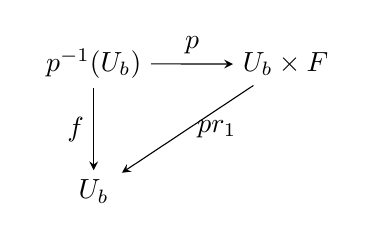
\begin{tikzpicture}
  \matrix (m) [matrix of math nodes,row sep=3em,column sep=3em,minimum width=2em]
  {
     {p^{-1}(U_b)} & {U_b \times F} \\
     U_b & \\};
  \path[-stealth]
    (m-1-1) edge node [above] {$p$}    (m-1-2)
            edge node [left]  {$f$}    (m-2-1)
    (m-1-2) edge node [right] {$pr_1$} (m-2-1);
\end{tikzpicture}
\end{center}
\end{definition}

\begin{definition} (Cartesian Product of Family over B).
Is a set $F$ of sections of the bundle with elimination map $app : F \times B \rightarrow E$ such that
\begin{equation}
F \times B \mapright{app} E \mapright{pr_1} B
\end{equation}
$pr_1$ is a product projection, so $pr_1$, $app$ are moriphisms
of slice category $Set_{/B}$. The universal mapping property of $F$:
for all $A$ and morphism $A \times B \rightarrow E$ in $Set_{/B}$ exists
unique map $A \rightarrow F$ such that everything commute. So a category
with all dependent products is necessarily a category with all pullbacks.
\end{definition}

\begin{definition} (Trivial Fiber Bundle).
When total space $E$ is cartesian product $\Sigma(B,F)$ and $p = pr_1$
then such bundle is called trivial $(F,\Sigma(B,F),pr_1,B)$.
\end{definition}

\begin{definition} (Dependent Product).
The dependent product along morphism $g: B \rightarrow A$ in category $C$ is the right
adjoint $\Pi_g : C_{/B} \rightarrow C_{/A}$ of the base change functor.
\end{definition}

\begin{definition} (Space of Sections).
Let $\mathbf{H}$ be a $(\infty,1)$-topos, and let $E \rightarrow B : \mathbf{H}_{/B}$ a bundle in
$\mathbf{H}$, object in the slice topos. Then the space of sections $\Gamma_\Sigma(E)$
of this bundle is the Dependent Product:
$$ \Gamma_\Sigma(E) = \Pi_\Sigma (E) \in \mathbf{H}. $$
\end{definition}

\begin{theorem} (Functions Preserve Paths).
For a function $f: (x:A) \rightarrow B(x)$
there is an $ap_f : Path_A(x,y) \rightarrow Path_{B(x)}(f(x),f(y))$. This is called
application of $f$ to path or congruence property (for non-dependent case ---
$cong$ function). This property behaves functoriality
as if paths are groupoid morphisms and types are objects.
\end{theorem}

\begin{theorem} (Trivial Fiber equals Family of Sets).
Inverse image (fiber) of fiber bundle $(F,B*F,pr_1,B)$ in point $y:B$ equals $F(y)$.
\begin{lstlisting}
FiberPi (B: U) (F: B -> U) (y: B)
      : Path U (fiber (Sigma B F) B (pi1 B F) y) (F y)
\end{lstlisting}
\end{theorem}

\begin{theorem} (Homotopy Equivalence).
If fiber space is set for all base, and
there are two functions $f,g : (x:A) \rightarrow B(x)$ and two
homotopies between them, then these homotopies are equal.
\begin{lstlisting}
setPi (A: U) (B: A -> U) (h: (x: A) -> isSet (B x)) (f g: Pi A B)
      (p q: Path (Pi A B) f g) : Path (Path (Pi A B) f g) p q
\end{lstlisting}
\end{theorem}

\begin{theorem} (HomSet).
If codomain is set then space of sections is a set.
\begin{lstlisting}
setFun (A B : U) (_: isSet B) : isSet (A -> B)
\end{lstlisting}
\end{theorem}

\begin{theorem} (Contractability).
If domain and codomain is contractible then the space of sections is contractible.
\begin{lstlisting}
piIsContr (A: U) (B: A -> U) (u: isContr A)
          (q: (x: A) -> isContr (B x)) : isContr (Pi A B)
\end{lstlisting}
\end{theorem}

\newpage
\subsection{Sigma}

$\Sigma$ is a dependent product type, the generalization of products.
$\Sigma$ type is a total space of fibration. Element of total
space is formed as a pair of basepoint and fibration. Also,
$\Sigma$ types is used to represent fiber space indexed by point in a base.

\begin{definition} (Formation).
\begin{lstlisting}
Sigma (A : U) (B : A -> U) : U = (x : A) * B x
\end{lstlisting}
\end{definition}

\begin{definition} (Introduction).
\begin{lstlisting}
dpair (A: U) (B: A -> U) (a: A) (b: B a) : Sigma A B = (a,b)
\end{lstlisting}
\end{definition}

\begin{definition} (Elimination).
\begin{lstlisting}
pr1 (A: U) (B: A -> U)
    (x: Sigma A B): A = x.1

pr2 (A: U) (B: A -> U)
    (x: Sigma A B): B (pr1 A B x) = x.2

sigInd (A: U) (B: A -> U) (C: Sigma A B -> U)
       (g: (a: A) (b: B a) -> C (a, b))
       (p: Sigma A B) : C p = g p.1 p.2
\end{lstlisting}
\end{definition}

\begin{definition} (Computation).
\begin{lstlisting}
Beta1 (A: U) (B: A -> U)
      (a:A) (b: B a)
    : Equ A a (pr1 A B (a,b))
    = refl A a

Beta2 (A: U) (B: A -> U)
      (a: A) (b: B a)
    : Equ (B a) b (pr2 A B (a,b))
    = reflect (B a)
\end{lstlisting}
\end{definition}

\begin{definition} (Uniqueness).
\begin{lstlisting}
Eta12 (A: U) (B: A -> U) (p: Sigma A B)
    : Equ (Sigma A B) p (pr1 A B p,pr2 A B p)
    = refl (Sigma A B) p
\end{lstlisting}
\end{definition}

\newpage
\subsubsection*{Examples from Mathematics}

\begin{definition} (Dependent Sum).
The dependent sum along the morphism $f: A \rightarrow B$ in category $C$ is the left
adjoint $\Sigma_f : C_{/A} \rightarrow C_{/B}$ of the base change functor.
\end{definition}

\begin{theorem} (Axiom of Choice).
If for all $x : A$ there is $y : B$ such that $R(x,y)$,
then there is a function $f : A \rightarrow B$
such that for all $x : A$ there is a witness of $R(x,f(x))$.
\begin{lstlisting}
ac (A B: U) (R: A -> B -> U)
 : (p: (x:A) -> (y:B)*(R x y)) -> (f:A->B) * ((x:A)->R(x)(f x))
\end{lstlisting}
\end{theorem}

\begin{theorem} (Total).
If fiber over base implies another fiber
over the same base then we can construct total space of section
over that base with another fiber.
\begin{lstlisting}
total (A:U) (B C: A -> U)
      (f: (x:A) -> B x -> C x) (w: Sigma A B)
    : Sigma A C = (w.1,f (w.1) (w.2))
\end{lstlisting}
\end{theorem}

\begin{theorem} ($\Sigma$-Contractability). If the fiber is set then the $\Sigma$ is set.
\begin{lstlisting}
setSig (A:U) (B: A -> U) (sA: isSet A)
       (sB : (x:A) -> isSet (B x)) : isSet (Sigma A B)
\end{lstlisting}
\end{theorem}

\begin{theorem} (Path Between Sigmas).
Path between two sigmas $t,u: \Sigma(A,B)$ could be decomposed to
sigma of two paths $p:t_1=_{A}u_1)$ and $(t_2=_{B(p@i)}u_2)$.
\begin{lstlisting}
pathSig (A:U) (B : A -> U) (t u : Sigma A B)
      : Path U (Path (Sigma A B) t u)
               ((p: Path A t.1 u.1) * PathP (<i>B(p@i)) t.2 u.2)
\end{lstlisting}
\end{theorem}

\newpage
\subsection{Path}

The Path identity type defines a Path space with elements and values.
Elements of that space are functions from interval $[0,1]$ to a values of that path space.
This ctt file reflects \footnote{Cyril Cohen, Thierry Coquand, Simon Huber, Anders M{\"{o}}rtberg. Cubical Type Theory: a constructive interpretation of the univalence axiom. 2015. \url{https://5ht.co/cubicaltt.pdf}}{CCHM} cubicaltt model with connections.
For \footnote{Carlo Angiuli, Brunerie, Coquand, Kuen-Bang Hou (Favonia), Robert Harper, Dan Licata. Cartesian Cubical Type Theory. 2017. \url{https://5ht.co/cctt.pdf}}{ABCFHL} yacctt model with
variables please refer to ytt file. You may also want to
read \footnote{Marc Bezem, Thierry Coquand, Robert Huber. A model of type theory in cubical sets. 2014. \url{http://www.cse.chalmers.se/~coquand/mod1.pdf}}{BCH},
\footnote{Carlo Angiuli, Kuen-Bang Hou (Favonia), Robert Harper. Cartesian Cubical Computational Type Theory: Constructive Reasoning with Paths and Equalities. 2018. \\ \url{https://www.cs.cmu.edu/~cangiuli/papers/ccctt.pdf}}{AFH}.
There is a \footnote{Andrew Pitts, Ian Orton. Axioms for Modelling Cubical Type Theory in a Topos. 2016. \url{https://arxiv.org/pdf/1712.04864.pdf}}{PO} paper about CCHM axiomatic in a topos.

\begin{definition} (Formation).
\begin{lstlisting}
HeteroPath (A B: U) (a: A) (b: B) (P: Path U A B) : U = PathP P a b
Path (A: U) (a b: A) : U = PathP (<i> A) a b
\end{lstlisting}
\end{definition}

\begin{definition} (Introduction).
Returns an element of reflexivity path space for a given value of the type.
The inhabitant of that path space is the lambda on the homotopy
interval $[0,1]$ that returns a constant value a. Written in
syntax as $<i>a = \lambda(i:I)\rightarrow a$.
\begin{lstlisting}
refl (A: U) (a: A) : Path A a a
\end{lstlisting}
\end{definition}

\begin{definition} (Path Application).
You can apply face to path.
\begin{lstlisting}
app1 (A: U) (a b: A) (p: Path A a b): A = p @ 0
app2 (A: U) (a b: A) (p: Path A a b): A = p @ 1
\end{lstlisting}
\end{definition}

\begin{definition} (Connections).
Connections allows you to build square
with given only one element of path: i) $\\(i,j:I) \rightarrow p\ @\ min(i,j)$;
ii) $\\(i,j:I)\rightarrow p\ @\ max(i,j)$.
\begin{center}
  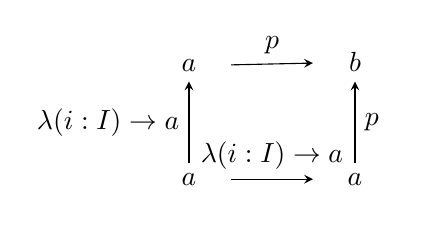
\begin{tikzpicture}
  \matrix (m) [matrix of math nodes,row sep=3em,column sep=3em,minimum width=3em]
  {
     a & b \\ % (1,1) (1,2)
     a & a                    \\ % (2,1) (2,2)
  };
  \path[-stealth]
    (m-1-1) edge node [above] {$p$}    (m-1-2)
    (m-2-1) edge node [left]  {$\lambda(i:I)\rightarrow a$}    (m-1-1)
    (m-2-2) edge node [right] {$p$} (m-1-2)
    (m-2-1) edge node [above] {$\lambda(i:I)\rightarrow a$} (m-2-2);
  \end{tikzpicture}
  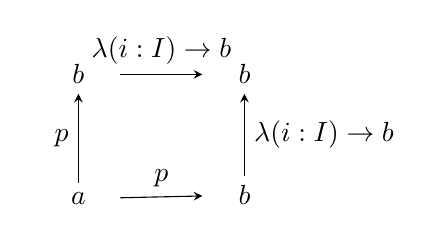
\begin{tikzpicture}
  \matrix (m) [matrix of math nodes,row sep=3em,column sep=3em,minimum width=3em]
  {
     b & b \\ % (1,1) (1,2)
     a & b                    \\ % (2,1) (2,2)
  };
  \path[-stealth]
    (m-1-1) edge node [above] {$\lambda(i:I)\rightarrow b$}    (m-1-2)
    (m-2-1) edge node [left]  {$p$}    (m-1-1)
    (m-2-2) edge node [right] {$\lambda(i:I)\rightarrow b$} (m-1-2)
    (m-2-1) edge node [above] {$p$} (m-2-2);
  \end{tikzpicture}
\end{center}
\begin{lstlisting}
connection1 (A: U) (a b: A) (p: Path A a b)
          : PathP (<x> Path A (p@x) b) p (<i>b)
          = <y x> p @ (x \/ y)

connection2 (A: U) (a b: A) (p: Path A a b)
          : PathP (<x> Path A a (p@x)) (<i>a) p
          = <x y> p @ (x /\ y)
\end{lstlisting}
\end{definition}

\begin{definition} (Composition).
Composition operation allows to build a new path by given to paths
in a connected point. The proofterm is $comp (<i>Path A a (q@i)) p []$.
\begin{center}
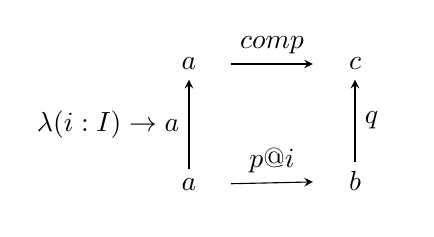
\begin{tikzpicture}
  \matrix (m) [matrix of math nodes,row sep=3em,column sep=3em,minimum width=3em]
  {
     a & c \\ % (1,1) (1,2)
     a & b \\ % (2,1) (2,2)
  };
  \path[-stealth]
    (m-1-1) edge node [above] {$comp$} (m-1-2)
    (m-2-1) edge node [left]  {$\lambda(i:I)\rightarrow a$} (m-1-1)
    (m-2-2) edge node [right] {$q$} (m-1-2)
    (m-2-1) edge node [above] {$p @ i$} (m-2-2);
\end{tikzpicture}
\end{center}
\begin{lstlisting}
composition (A: U) (a b c: A)
            (p: Path A a b) (q: Path A b c) : Path A a c
\end{lstlisting}
\end{definition}

\begin{theorem} (Congruence).
Is a map between values of one type
to path space of another type by an encode function between types.
Implemented as lambda defined on $[0,1]$ that returns
application of encode function to path application of
the given path to lamda argument $\lambda(i:I)\rightarrow f (p @ i)$
for both cases.
\begin{lstlisting}
ap  (A B: U) (f: A -> B)
    (a b: A) (p: Path A a b)
  : Path B (f a) (f b)

apd (A: U) (a x:A) (B:A->U) (f: A->B a)
    (b: B a) (p: Path A a x)
  : Path (B a) (f a) (f x)
\end{lstlisting}
\end{theorem}

\begin{theorem} (Transport).
Transports a value of the domain type to the value of the codomain type
by a given path element of the path space between domain and codomain types.
Defined as path composition with $[]$ of a over a path $p$ --- $comp p a []$.
\begin{lstlisting}
trans (A B: U) (p: Path U A B) (a: A) : B
\end{lstlisting}
\end{theorem}


\begin{theorem} (Eliminator, Paulin-Mohring).
J is formulated in a form of Paulin-Mohring and implemented using
two facts that singleton are contractible and dependent function
transport.
\begin{lstlisting}
J (A: U) (a b: A)
  (P: singl A a -> U)
  (u: P (a,refl A a))
  (p: Path A a b) : P (b,p)
\end{lstlisting}
\end{theorem}

\begin{theorem} (Eliminator, HoTT).
J from HoTT book.
\begin{lstlisting}
J (A: U) (a b: A)
  (C: (x: A) -> Path A a x -> U)
  (d: C a (refl A a))
  (p: Path A a b) : C b p
\end{lstlisting}
\end{theorem}

\begin{theorem} (Eliminator, Diagonal).
\begin{lstlisting}
D (A: U) : U = (x y: A) -> Path A x y -> U
J (A: U) (x y: A) (C: D A)
  (d: C x x (refl A x))
  (p: Path A x y) : C x y p
\end{lstlisting}
\end{theorem}

\begin{theorem} (Computation).
\begin{lstlisting}
trans_comp (A: U) (a: A)
  : Path A a (trans A A (<_> A) a)
subst_comp (A: U) (P: A -> U) (a: A) (e: P a)
  : Path (P a) e (subst A P a a (refl A a) e)
J_comp (A: U) (a: A) (C: (x: A) -> Path A a x -> U) (d: C a (refl A a))
  : Path (C a (refl A a)) d (J A a C d a (refl A a))
\end{lstlisting}
\end{theorem}

%\section{Inductive Types}
%\subsection{Empty}
%\subsection{Unit}
%\subsection{Bool}
%\subsection{Either}
%\subsection{Nat}
%\subsection{List}
%\subsection{Fin}
%\subsection{Vector}
\section{Homotopy Type Theory}
%\subsection{n-Types}
\subsection{Functional Extensionality}

\begin{definition} (Formation).
\end{definition}

\begin{theorem} (Introduction).
\end{theorem}

\begin{theorem} (Elimination).
\end{theorem}

\begin{theorem} (Computation).
\end{theorem}

\begin{theorem} (Uniqueness).
\end{theorem}

%\subsection{Univalence}

%\begin{definition} (Formation).
%\end{definition}

%\begin{theorem} (Introduction).
%\end{theorem}

%\begin{theorem} (Elimination).
%\end{theorem}

%\begin{theorem} (Computation).
%\end{theorem}

%\begin{theorem} (Uniqueness).
%\end{theorem}

%\section{Higher Inductive Types}
%\subsection{Interval}
%\subsection{$S^1$}
%\subsection{Pullback}
%\subsection{Pushout}
%\subsection{Truncation}
%\subsection{Quotient}
%\subsection{Loop Space}
%\subsection{Homotopy Group}
%\section{Cohesive Type Theory}
%\subsection{Fundametal $\infty$-Groupoid}
%\subsection{Infinitesimal Modality}
%\subsection{Sharp Modality}
%\subsection{Formal Disc}
%\subsection{Etale Maps}
%\subsection{Manifolds}

%\newpage
\bibliographystyle{plain}
\bibliography{types}

\end{document}

